\documentclass[man]{apa7}
\usepackage{lipsum}
\usepackage[american]{babel}
\usepackage{csquotes}
\usepackage{hyperref}
\usepackage{float}
\usepackage[style=apa,sortcites=true,sorting=nyt,backend=biber]{biblatex}
\DeclareLanguageMapping{american}{american-apa}
\addbibresource{references.bib}


\title{The puzzling relationship between multi-lab replications and 
meta-analyses of the published literature
}
\shorttitle{Multi-lab replications and meta-analytic effect sizes}
\author{Molly Lewis$^{1}$, Maya B. Mathur$^{2}$, Tyler J. VanderWeele$^{3}$, and Michael C. Frank$^{2}$}
\affiliation{$^{1}$Carnegie Mellon University\\
$^{2}$Stanford University\\
$^{3}$Harvard University\\}


\abstract{What is the best way to estimate the size of important effects? Should we aggregate across disparate findings using statistical meta-analysis, or instead run large, multi-lab replications (MLR)? A recent paper by Kvarven, Strømland, and Johannesson (2020) compared effect size estimates derived from these two different methods for 15 different psychological phenomena.  The authors report that, for the same phenomenon, the meta-analytic estimate tends to be about three times larger than the MLR estimate.  These results pose an important puzzle:  What is the relationship between these two estimates? Kvarven et al.\ suggest that their results undermine the value of meta-analysis. In contrast, we argue that both meta-analysis and MLR are informative, and that the discrepancy between estimates obtained via the two methods is in fact still unexplained. Informed by re-analyses of Kvarven et al.'s data and by other empirical evidence, we discuss possible sources of this discrepancy and argue that understanding the relationship between estimates obtained from these two methods is an important puzzle for future meta-scientific research.  }
\keywords{meta-analysis, multi-lab replication, meta-science}

\authornote{
  Correspondence concerning this article should be addressed to Molly Lewis, Psychology Department, Carnegie Mellon University.  E-mail: mollylewis@cmu.edu}

\begin{document}
\maketitle

%\section{Introduction}

Obtaining precise and unbiased estimates of the sizes of experimental effects is an important goal in both theory and application in psychological science. Such estimates can be used for the development and testing of quantitative models, leading to more robust theories \parencite{oberauer2019addressing}. Further, precise and unbiased estimates of intervention effects are critical for decision-making in applied contexts. Unfortunately, studies run in individual labs are rarely able to accumulate the sample sizes necessary to provide adequate precision \parencite{simonsohn_2014}, and furthermore individual studies may be subject to substantial publication bias.  There is thus a critical need for alternative estimation methods. 

Statistical meta-analysis \parencite{gurevitch2018meta,dersimonian1986meta} has become the de facto standard for estimating effect sizes in important cases. Indeed, evidence pyramids often treat meta-analysis as one of the most credible forms of evidence, indicating the trust that is put on these quantitative summaries of the literature \parencite{higgins2019cochrane}. Yet in recent years, psychology has experienced a crisis of confidence in its prior literature, brought on by empirical reports that show low levels of replication for many prominent findings in the prior literature \parencite{open2015estimating,klein2014investigating,klein2018many,ebersole2016many}. Such failures to replicate may be due in part to “questionable research practices” on the part of individual researchers \parencite[e.g., post-hoc analytic decision-making;][]{masicampo2012peculiar} and a bias for findings to be published only if they meet a significance threshold. Meta-analyses that include highly biased findings may thus be suspect as sources of accurate effect estimates  \parencite[or even as indicators of whether an effect is consistently non-zero;][]{vadillo2016selection}. 

An alternative method for estimating effects accurately is to conduct large, multi-lab replication (MLR) studies. Such studies provide precise estimates by enlisting many labs to contribute data, leading to unusually large sample sizes (by the standards of previous literature). Further, such replication attempts are typically pre-registered, reducing bias in their effect estimates by removing analytic flexibility \parencite{nosek2018preregistration}. 

The presence of these two distinct routes for estimating important experimental effects naturally leads to a question. In cases of uncertainty, how much relative confidence should we place on aggregated findings using statistical meta-analysis versus large, multi-lab replications?  

\section{Empirical comparisons of meta-analyses and MLRs}

A recent paper by Kvarven, Strømland, and Johannesson (henceforth \textit{KSJ}; 2020) compared effect size estimates derived from these two different methods for 15 different psychological phenomena. Na{\"i}vely, we might expect that if studies in a meta-analysis and the corresponding MLR are measuring identical phenomena, and there is no analytical or publication bias, the effect size estimates obtained via the two methods should be similar.  In contrast, KSJ report that, for the same phenomenon, the meta-analytic estimate tends to be about three times larger than the MLR estimate. KSJ suggest that their results undermine the value of meta-analysis. In contrast, we argue that both meta-analysis and MLR are informative but that the relationship between them is an important puzzle for future meta-research. 

To conceptualize the tradeoffs between meta-analysis and MLR, it helps to consider different scenarios. In the most extreme case, in which the prior literature is stipulated to be extremely biased (perhaps due to cases of extreme analytic flexibility leading to a literature comprised only of false positives), it’s easy to see that meta-analysis would be worthless; MLR would be the optimal method for obtaining a precise estimate of the size of an experimental effect \parencite[for a possible example of this type, see e.g.][]{vadillo2016selection}. On the other hand, if the prior literature includes some genuine positive results (even alongside some false positives), the meta-analysis will have at least some value. 

Are we usually in this first scenario? KSJ show that meta-analysis and MLR produce divergent estimates of effect size, but this result does not necessarily undermine the value of meta-analysis or indicate that the prior literature is composed exclusively of false positives. There may be genuine and substantive reasons for differences between MLR and meta-analysis estimates. Indeed, examining KSJ’s data, there is a strong relationship between effect size estimates from the MLR and the meta-analyses: Phenomena with larger meta-analytic estimates tend to also have larger estimates in the MLR (Pearson’s $r$ = 0.72 [0.32, 0.90], $p$ = 0.003; Fig.\ 1). Thus, although meta-analyses do show larger effects, they are not uninformative regarding the results of MLR. Hence we can infer that KSJ’s sample of findings are not generated from a world in which the prior literature is worthless. 

\begin{figure}[H]
\centering
     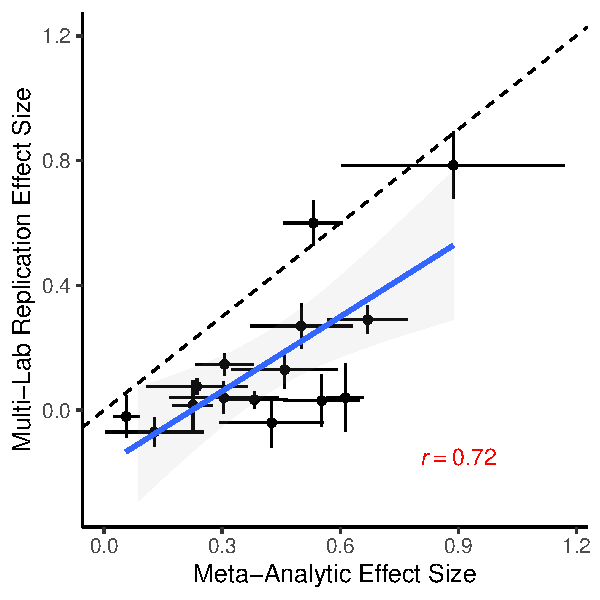
\includegraphics[width=5in]{figs/fig1a.pdf}
      \caption{  Correlation between effect size estimates from multiple-laboratory replications and random effect meta-analytic estimates (Pearson’s $r$(13) = 0.72 [0.32, 0.9], $p$ = 0.003). Each point corresponds to a phenomenon ($N$ = 15), and ranges indicate 95\% confidence intervals. The dashed reference line has a slope of 1. }
\end{figure}


\section{Genuine effect heterogeneity may explain some of the discrepancy}

Further, many of the meta-analyses in KSJ’s study showed considerable effect heterogeneity. When effects are heterogeneous, a comparison of the meta-analytic mean to the MLR mean---KSJ’s primary comparison---does not, on its own, adequately characterize the evidence for a true difference between the two \parencite{mathur2019new}. Comparing only the means of potentially heterogeneous effect distributions can in fact create a false impression of conflict when in fact little conflict exists \parencite{mathur2019new, mathur2019finding}. 

To test this idea, we examined where each MLR mean would fall in the distribution of population effects in the corresponding meta-analysis \parencite{mathur2020robust}. We estimated that, across meta-analyses, a median  of 20\% of the population effects in the meta-analyzed studies were at least as small as the corresponding MLR mean estimate (Fig.\ 2, right-hand side). Thus, although \emph{average} effect sizes were typically larger in meta-analyses versus MLRs, it was often the case that a sizeable minority of the effects in the meta-analyses were in fact well within the distribution of effects in the corresponding MLR, perhaps indicating a smaller discrepancy than is apparent when comparing only the means. Such heterogeneity could arise from variation across studies in, for example, sample settings and protocols.

\begin{figure}[t]
\centering
     \includegraphics[width=7in]{figs/forest.pdf}
      \caption{Estimates from sensitivity analyses representing worst-case publication bias (vertical tick marks with 95\% confidence intervals [CI]) versus naïve meta-analysis estimates (diamonds) and multi-lab replication estimates (MLR; circles). Meta-analyses are ordered by their naïve estimates. For orange-colored meta-analyses, the worst-case estimate exceeds the MLR estimate, indicating that no amount of publication bias that purely favors statistically significant and positive results could entirely explain the discrepancy between the naïve estimate and the MLR estimate. Percentages and 95\% CIs on the right-hand side represent the estimated percentage of true population effects in the naïve meta-analysis that are as small as, or smaller than, the MLR estimate. CIs are omitted when they were not estimable via bias-corrected and accelerated bootstrapping \parencite{mathur2020robust}.}
\end{figure}

Although the discrepancy between meta-analysis and MLR results is thus perhaps smaller than KSJ suggest, a discrepancy does still exist. Effect heterogeneity alone does not fully account for the differences. What is the source of the remaining discrepancy? 

\section{Publication bias cannot entirely explain the discrepancy}

KSJ speculate that the MLR/meta-analysis discrepancy is likely due to “questionable research practices” \parencite{masicampo2012peculiar} such as post-hoc analytic decision-making or publication bias. Both of these practices act as filters that select for statistically significant findings, leading to an inflation of effect size. Could these mechanisms be fully responsible? 

One way to address this question is to estimate the meta-analytic effect size correcting for publication bias. KSJ did so using several different statistical methods, which typically still yielded estimates that were considerably larger than the MLR estimates. KSJ therefore concluded that the statistical methods are themselves flawed and ``ineffective in fully adjusting inflated effect sizes for publication bias.'' That principled statistical adjustments \parencite{vevea1995general} do not eliminate the systematic discrepancy between the meta-analysis and MLR estimates must reflect either: (1) that statistically adjusted meta-analysis estimates were indeed badly biased due to serious violations of the methods' assumptions, or alternatively (2) that the statistically adjusted meta-analysis estimates were not, in fact, badly biased, because there are fundamental substantive reasons, not merely publication bias, for effect sizes to genuinely differ between meta-analyses and MLRs.  

To help adjudicate between these two possibilities, we conducted a re-analysis that uses a fundamentally different approach called ``sensitivity analysis'' \parencite{mathur2019sensitivity}. In contrast to the methods used by KSJ, the sensitivity analysis methods correct the estimate not by attempting to estimate the actual severity of publication bias present in the meta-analysis, but rather by considering only hypothetical worst-case publication bias by essentially ignoring all statistically significant results in the expected direction \parencite{mathur2019sensitivity}. In doing so, these methods provide a highly conservative estimate and obviate many (though not all) of the assumptions of standard methods that might in principle have caused them to adjust inadequately.

The methods we used assume a model of publication bias in which  statistically significant positive studies (``affirmative studies'') are more likely to be published than nonsignificant and/or negative studies (``non-affirmative studies''), and there is no further selection based on the size of the point estimate or on characteristics associated with the point estimate (such as the $p$-value treated as continuous, rather than dichotomized at $\alpha$ = 0.05). This model of publication bias is identical to that assumed by the three-parameter selection model used by KSJ \parencite{vevea1995general}, and it conforms well to empirical evidence regarding how publication bias operates in practice \parencite{mathur2019sensitivity}. However, unlike the three-parameter selection models used in KSJ, the present methods do not require a large number of meta-analyzed studies and do not make any distributional assumptions. ``Publication bias'' in this context could reflect the aggregation of multiple sources of bias, including, for example, investigators’ selective reporting of experiments or preparation of papers for submission as well as journals’ selective acceptance of papers. 

To provide some intuition for how the sensitivity analysis methods work, if the degree of publication bias were known, a bias-corrected meta-analytic estimate could hypothetically be obtained by upweighting the contribution of each nonaffirmative study in the meta-analysis by the same ratio by which the publication process favors affirmative studies. For example, suppose it were known that affirmative results were five times more likely to be published than nonaffirmative studies and that, given a study’s nonaffirmative or affirmative status, the publication process did not select further based on the size of the point estimate. Then the point estimates of the published nonaffirmative studies (i.e., those included in the meta-analysis) would be essentially a random sample of those from the larger, underlying population of nonaffirmative studies, most of which are not published. A bias-corrected meta-analytic estimate could therefore be obtained by upweighting the contribution of each nonaffirmative study in the meta-analysis by fivefold to counteract the publication process’ fivefold favoring of affirmative studies.

Since the degree of publication bias is not exactly known in practice, the sensitivity analyses can also estimate the meta-analytic mean under a hypothetical “worst-case” publication bias scenario \parencite{mathur2019sensitivity}, in which affirmative studies are infinitely more likely to be published than nonaffirmative studies.  That is, worst-case publication bias would effectively favor affirmative studies by an infinite ratio, so a worst-case estimate can be obtained by meta-analyzing only the nonaffirmative studies that are included in the meta-analyses and simply discarding the affirmative studies. Intuitively, this method works because such an analysis is effectively equivalent to upweighting each nonaffirmative study by a factor of infinity. Such a worst-case analysis does not require actual estimation of the ratio by which the publication process favors affirmative studies.
 
We conducted this sensitivity analysis for the KSJ data by analyzing the 13 of 15 meta-analyses for which the meta-analytic mean estimate was larger than the MLR estimate and for which these analyses were statistically feasible (meta-analyses must contain at least one nonaffirmative study). For the majority of such meta-analyses (62\%), even worst-case publication bias of this nature could not attenuate the meta-analytic estimate to match that of the MLR. Also, for all but one of these meta-analyses (i.e. 92\%), worst-case publication bias could not attenuate the meta-analytic estimate all the way to the null (Fig.\ 2). In other words, even non-significant studies -- which shouldn't be subject to publication bias -- showed effects that were greater than zero and greater than the MLR estimate. It therefore appears somewhat implausible that a realistic mechanism of publication bias, no matter how severe, could entirely explain the discrepancy between meta-analytic and MLR effect size estimates.

\section{Possible explanations for the remaining discrepancy}

What, then, are other possible causes of the discrepancy? One possibility is that the phenomena being studied may be sensitive to the details of the experimental materials and methods, and especially to how these interact with the specific populations being assessed. While this kind of method- and context-sensitivity has frequently been cited as a specifically post-hoc explanation for direct replication failures \parencite{van2016contextual}, a series of pre-registered replications that we and our collaborators have carried out attest to the importance of small methodological factors in replicating effects \parencite{lewis2018still,lewis2016understanding,phillips2015second}. 

For example, in \Textcite{lewis2016understanding}, we ran a series of five replications with minor methodological differences. While the first of these yielded an effect estimate close to zero, a series of subtle modifications led to a meta-analytic effect size estimate of about .5 (Cohen's $d$). The effect size in the last (preregistered) study (.71) was more than 4 times that of the first study (.17).   Across studies,  an estimate of the heterogeneity in the sample,  $\tau^{2}$ (.04), was within the range found in the sample of meta-analyses reported by KSJ (0 - .54; $M$ = .11). Notably, we observed this effect size variability in a case where the experiment was motivated by a formal model \parencite{xu2007word}, and where the methodological modifications were theory-irrelevant (e.g., online vs. in lab; exact stimuli used). The fact that we find this variability, despite the tight link between theory and experiment \parencite{oberauer2019addressing}, is particularly suggestive that small methodological decisions about the implementation of individual experiments can substantially influence the meta-analytic effect size, and that methodological variability may account for some of the discrepancy between MLR and meta-analytic effect size estimates.

Further, subtle methodological choices of individual studies within a meta-analysis may interact with the population of participants in an experiment, and investigators who are committed to understanding a particular phenomenon may take pains to tailor their stimuli to a particular context. Perhaps this is one reason that the individual studies in a meta-analysis typically vary considerably in their methods and stimuli. In contrast, MLRs typically standardize their materials across all populations and contexts being studied in order to establish a single method for all participating labs. This difference could account for some of the discrepancy in effect sizes. 

For example, one of the phenomena included in KSJ’s paper is an effect whereby imagining interaction with an outgroup member leads participants to be more likely to express an intention to engage with an outgroup member in real life. In the original paper \parencite{husnu2010elaboration}, the participants were British non-Muslim undergraduates, and the “outgroup” was British Muslims. In the corresponding MLR, 34 out of the 35 replication sites used the same outgroup, “Muslim,” despite the fact that the sites spanned nine different countries with likely varying degrees of prejudice toward Muslims. In contrast, in the meta-analysis, individual studies used a wide range of outgroups, adapted to the local social context of each study. Furthermore, even if labs were to likewise alter the stimuli according to context, individual studies may be more likely than MLR's to select samples and exclusion criteria to maximize effect sizes.

More broadly, and in social psychology especially, effects could well be more context sensitive relative to other psychological domains \parencite{van2016contextual,inbar2016association}. Notably, the majority of phenomena in KSJ concern effects that appear social or contextually-dependent (e.g., interactions between political belief and moral decision-making, humor responses, imagined intergroup contact, expression of prejudice). However, to carry empirical weight, speculations about context-sensitivity must be tested directly in future meta-scientific work. 

A final hypothesis about  the discrepancy between meta-analysis and MLR may be that in individual studies, as compared with MLRs, investigators may make greater (or more effective) efforts to ensure intervention fidelity, thereby increasing effect sizes. Such differences in fidelity would constitute investigator bias; instead under such circumstances, the interventions themselves would effectively be different (e.g., because participants received greater encouragement to engage). Such differences could be due to experimenter expertise, though meta-scientific attempts to find effects of expertise on replication success have been unsuccessful \parencite{open2015estimating}. More plausibly in our mind, differences could be due to feeling of “having more at stake” by original investigators relative to the myriad teams participating in a MLR effort, who may assume that a protocol being distributed to them should “just work.” (We write this characterization as participants in a variety of MLR efforts). 

\section{Conclusions}

In summary, building good scientific theories relies on having precise estimates of effect sizes, but the best way to obtain these estimates is not obvious. Both meta-analysis and MLRs provide methods for estimating the effect size of important phenomena by aggregating evidence across multiple studies. KSJ present the first systematic comparison of these two methods and show that effect sizes derived from meta-analyses are puzzlingly larger than those derived from MLRs. We demonstrate that meta-analytic effect sizes are related to MLR estimates, but there is still a remaining discrepancy between the two methods. Further, our analyses suggest that effect size heterogeneity and publication bias may contribute to---but are unlikely to account fully for---this discrepancy. Speculative possibilities for the remaining discrepancy include that MLRs obtain smaller effect sizes because of standardization of methods across labs (perhaps especially for context-sensitive phenomena) and because of the potential for differential effort to ensure intervention fidelity comparing MLRs and original literature. Understanding the source of the discrepancy between effect sizes estimated from meta-analyses and those from MLRs is an important, complex question for future meta-scientific research. 

\nocite{kvarven2020comparing} 


\section{Data availability}
\noindent Data and code for all analyses can be found in a repository for the project: \href{https://github.com/mllewis/kvarven_reanalysis/}{https://github.com/mllewis/kvarven\_reanalysis}

\section{Acknowledgments} 
\noindent Eirik Str{\o}mland provided forthcoming answers to our questions about his paper. We thank Martin Hagger for a thought-provoking discussion.

\newpage



\pagebreak

\printbibliography
\end{document}
